%%%%%%%%%%%%%%%%%%%%%%%%%%%%%%%%%%%%%%%%%%%%%%%%%%%%%%%%%%%%%%%%%
% Tese de Doutorado / Dept Fisica, CFM, UFSC                    %
% Andre@UFSC - 2014                                             %
%%%%%%%%%%%%%%%%%%%%%%%%%%%%%%%%%%%%%%%%%%%%%%%%%%%%%%%%%%%%%%%%%

%:::::::::::::::::::::::::::::::::::::::::::::::::::::::::::::::%
%                                                               %
%                          Capítulo 6                           %
%                                                               %
%:::::::::::::::::::::::::::::::::::::::::::::::::::::::::::::::%

%***************************************************************%
%                                                               %
%         Testes da decomposição morfológica espectral          %
%                                                               %
%***************************************************************%

\chapter{Testes da decomposição morfológica espectral}

\section{Construindo uma galáxia}

\section{Dependência do ajuste com  a PSF}
\label{sec:test:psf}

\section{Teste antigo (só pra referência, apagar depois!)}

Para determinar se o método de decomposição funciona (ou melhor, se ele falha
mesmo para o caso mais básico), foi desenhado um exercício bastante simples.
Dado um conjunto de parâmetros morfológicos arbitrários, foi montado um cubo de
espectros de uma galáxia sintética composta de um bojo velho (utilizando uma SSP
de $12\,Gyr$) e um disco jovem (utilizando uma SSP de $3\,Gyr$). Os espectros de
base para o bojo e o disco podem ser vistos na Figura \ref{fig:testSpectra}.
Após gerar os cubos de dados de espectros, foi adicionado um ruído gaussiano de
$10\%$. Executando a decomposição neste cubo de dados simulado, deveria-se
encontrar valores para os parâmetros próximos aos escolhidos no início. A Figura
\ref{fig:testParameters} mostra a comparação dos parâmetros obtidos com os
iniciais. Os valores ajustados (linhas sólidas) estão de acordo com o valor
inicial, levando em conta o erro injetado nos espectros. É necessário repetir
este teste com configurações mais complexas, a fim de determinar as limitações
do método.


\begin{figure}
	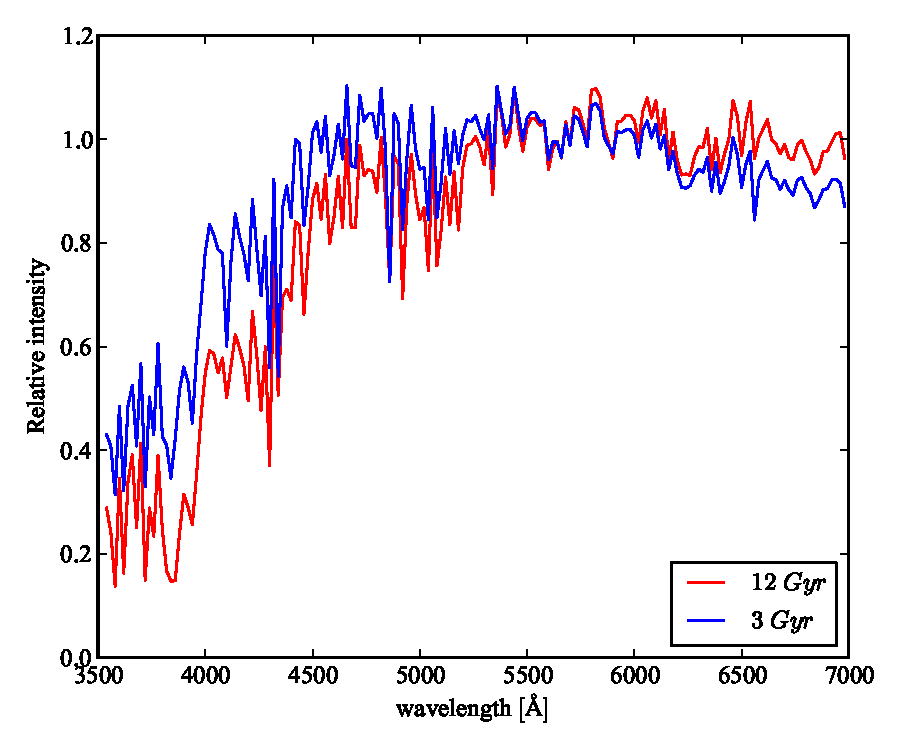
\includegraphics[width=0.7\columnwidth]{figuras/test-spectra}
	\caption[Espectros de base para o teste de decomposição] {Espectros de base
	para o teste de decomposição.}
	\label{fig:testSpectra}
\end{figure}


\begin{figure}
	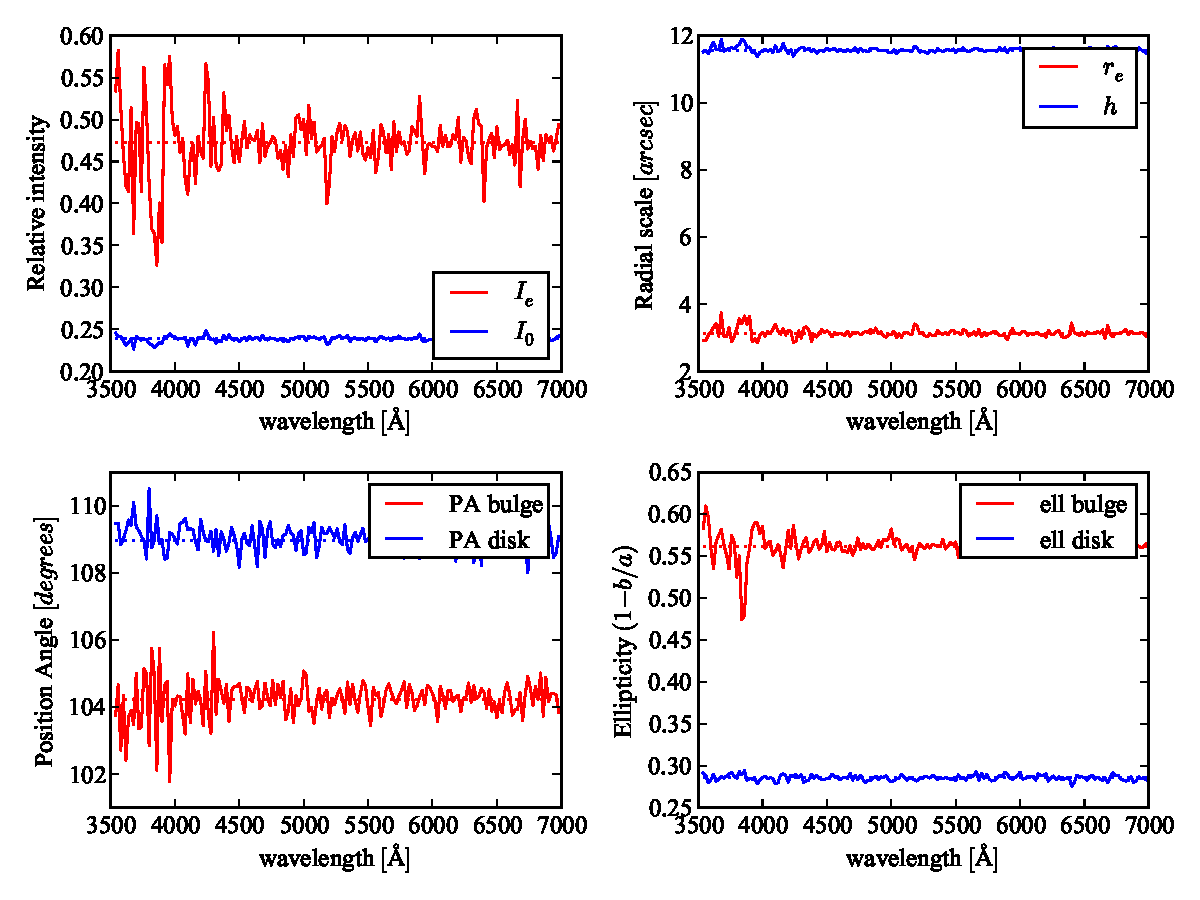
\includegraphics[width=1.0\columnwidth]{figuras/test-parameters}
	\caption[Parâmetros obtidos com o teste de decomposição] {Parâmetros obtidos
	com o teste de decomposição. Em tracejado são os parâmetros originais, em
	linhas sólidas os ajustes. Os parâmetros do bojo estão em vermelho e os do
	disco em azul. O índice de Sérsic ($n$) foi mantido constante e igual a $4$.}
	\label{fig:testParameters}
\end{figure}


%% End of this chapter
